\documentclass[12pt, a4paper, onecolumn]{article}
\usepackage{fontspec}
\usepackage{titlesec}
\usepackage{tocloft}
\usepackage[english]{babel}
\usepackage{blindtext}
\usepackage{subfig}
\usepackage{pgf}
\setmainfont{Georgia}
\usepackage{parskip}
\usepackage{float}

\newcommand\sectionfont{\normalfont\fontspec{Arial}\fontsize{14pt}{0}\bfseries}
\newcommand\subsectionfont{\normalfont\fontspec{Arial}\fontsize{13pt}{0}\bfseries}
\newcommand\subsubsectionfont{\normalfont\fontspec{Arial}\fontsize{12pt}{0}\bfseries}
\newcommand\tocsectionfont{\normalfont\fontspec{Arial}\fontsize{12pt}{0}\bfseries}
\newcommand\tocsubsectionfont{\normalfont\fontspec{Arial}\fontsize{11pt}{0}\bfseries}
\newcommand\tocsubsubsectionfont{\normalfont\fontspec{Arial}\fontsize{11pt}{0}}
\newcommand\toctitlefont{\normalfont\fontspec{Arial}\fontsize{16pt}{0}\bfseries}

\titleformat{\section}{\sectionfont}{\thesection}{20pt}{}
\titleformat{\subsection}{\subsectionfont}{\thesubsection}{20pt}{}
\titleformat{\subsubsection}{\subsubsectionfont}{\thesubsubsection}{20pt}{}

\renewcommand{\cftsecfont}{\tocsectionfont}
\renewcommand{\cftsubsecfont}{\tocsubsectionfont}
\renewcommand{\cftsubsubsecfont}{\tocsubsubsectionfont}
\renewcommand{\cftsecpagefont}{\tocsectionfont}
\renewcommand{\cftsubsecpagefont}{\tocsubsectionfont}
\renewcommand{\cftsubsubsecpagefont}{\tocsubsubsectionfont}
\renewcommand{\cfttoctitlefont}{\toctitlefont}

\newcommand{\parag}[1]{
	\textbf{#1} \hspace{0pt} \\
}

\addto\captionsenglish{
	\renewcommand{\contentsname}{Table of Contents}
}

\begin{document}

\section{Result}
		\subsection{Implementing a neural network}
			The implementation of the neural network consists of three steps. The first step is related to data collection. The second step involves designing the network in terms on layers and neurons, \textit{this will from now on be referenced as the model}, as well as fitting and evaluating the model to make as accurate predictions as possible. The final step using the model in the application and evaluate its accurateness in real world scenarios. The full process from data collection to final model can be seen in figure \ref{fig:training-model}.
			
			\begin{figure}[H]
				\centering
				\subfloat{{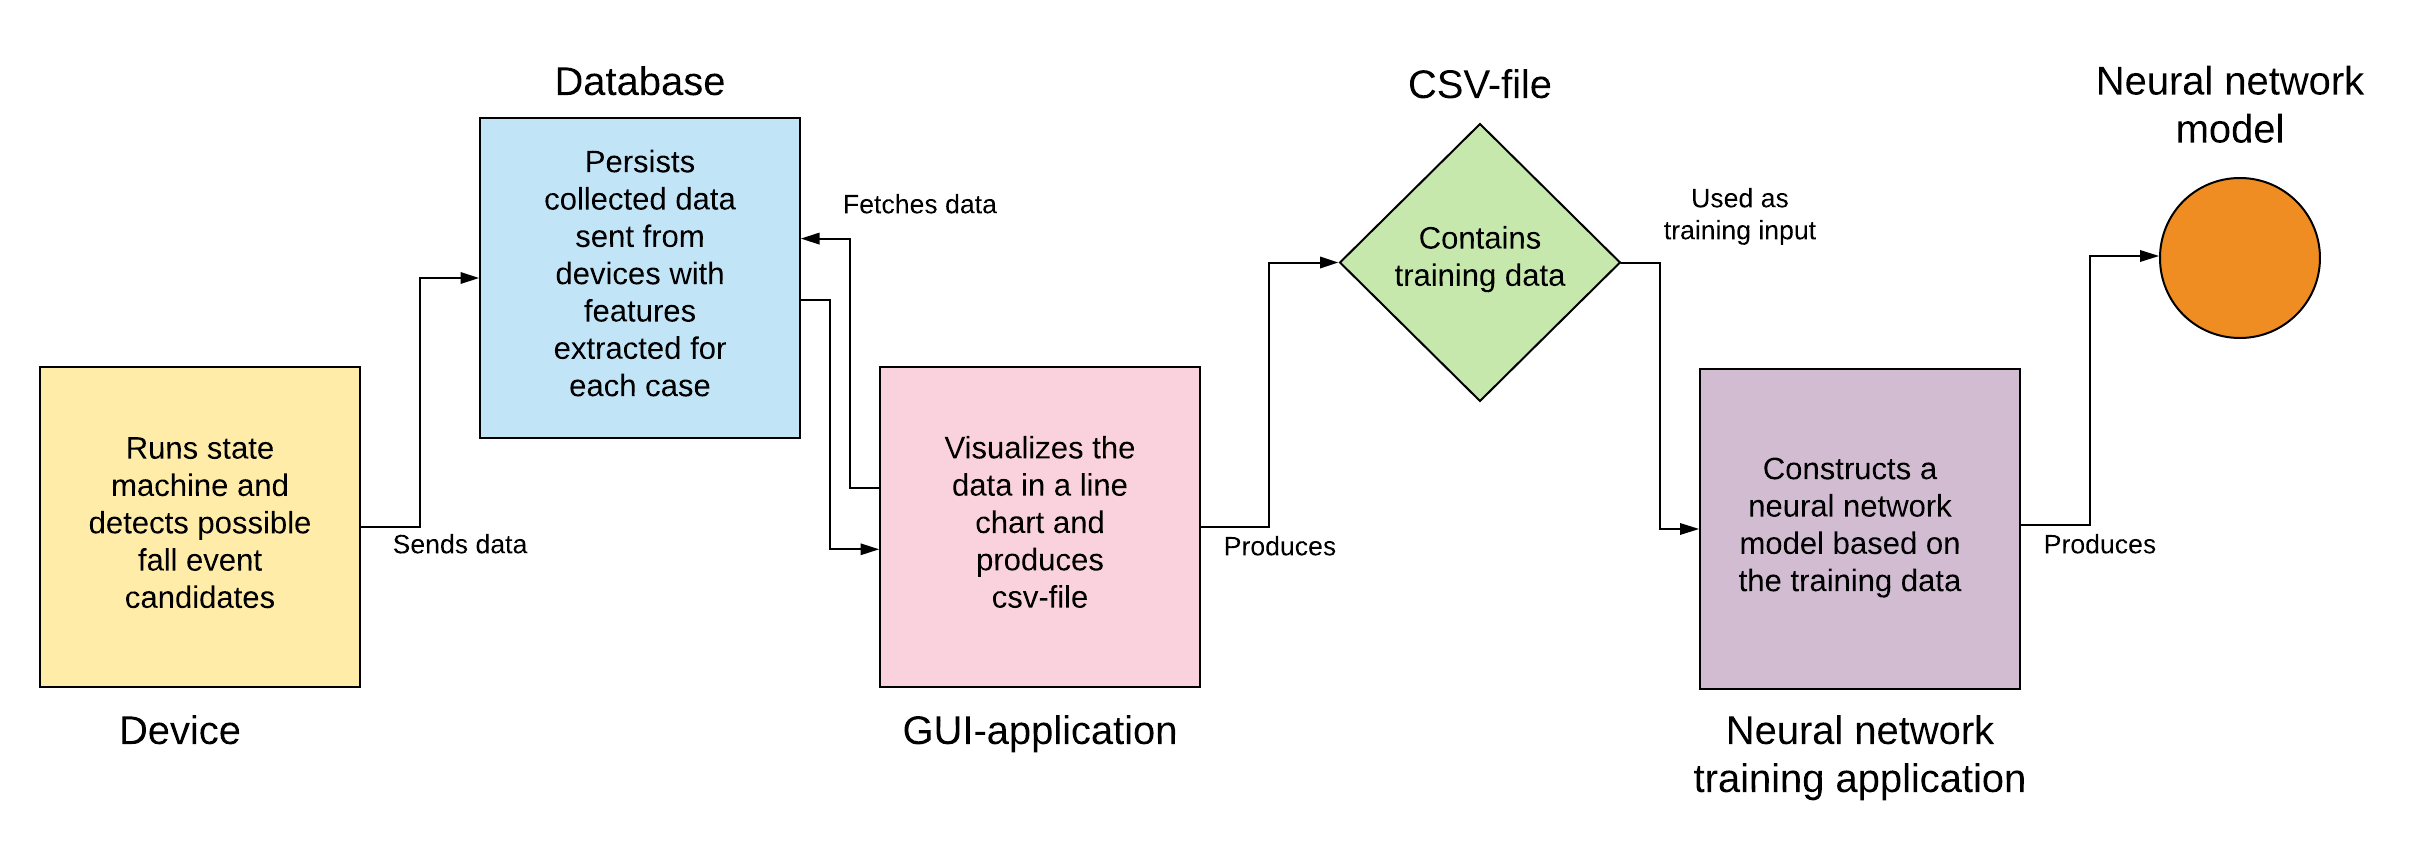
\includegraphics[width=15cm]{../img/training-model.png} }}%
				\caption{The process of collecting data and training the model}%
				\label{fig:training-model}%
			\end{figure}
			
		\subsubsection{Data collection}
		In order to collect motion data, we intercept every event that passed through our state-machine and following feature-extractor described in \textit{5.3} and \textit{5.4}. Thus, for all events that are recognized as a potential fall candidate, we have an object with its own set of the eight features described in \textit{5.4} as well as the original 400 sample long array of acceleration data collected from the accelerometer. The features are to be used when training the model and the array of data points is only used for visualization of the event on our graphical tool. Each event is labeled according to the class is belongs to \textit{fall, run/walk, jump}). The last step is to save each event to a database. 
		
		When collecting data for the \textit{run/walk} and \textit{jump} classes, we placed the device in the trouser pocket (\textit{a normal place to keep the device in everyday life}) and walked, ran and jumped respectively. Collecting data for the \textit{fall} class was done by letting the phone fall from different altitudes ranging from 1,5 m up to 3 m and landing on different natural surfaces. A series of events simulating falling while walking was also done by simply walking/running with the device and drop it to the ground mid walk.
		
		In total, 210 samples were collected, evenly distributed between the different classes and devices.

		\subsubsection{Designing a model}
			The neural network is built using \textit{Tensor Flow}, \textit{Keras} and the \textit{Python} programming language. After experimentation with the amount of hidden layers and neurons when training the model we arrived at the conclusion that a single hidden layer with seven neurons yielded the best possible accuracy given our data set. The activation function is set to \textit{sigmoid} for the hidden layer as well as the output layer. The result is a neural network with eight inputs, one for each feature, and three outputs, one for each class. 
			
			\begin{figure}[H]
				\centering
				\subfloat{{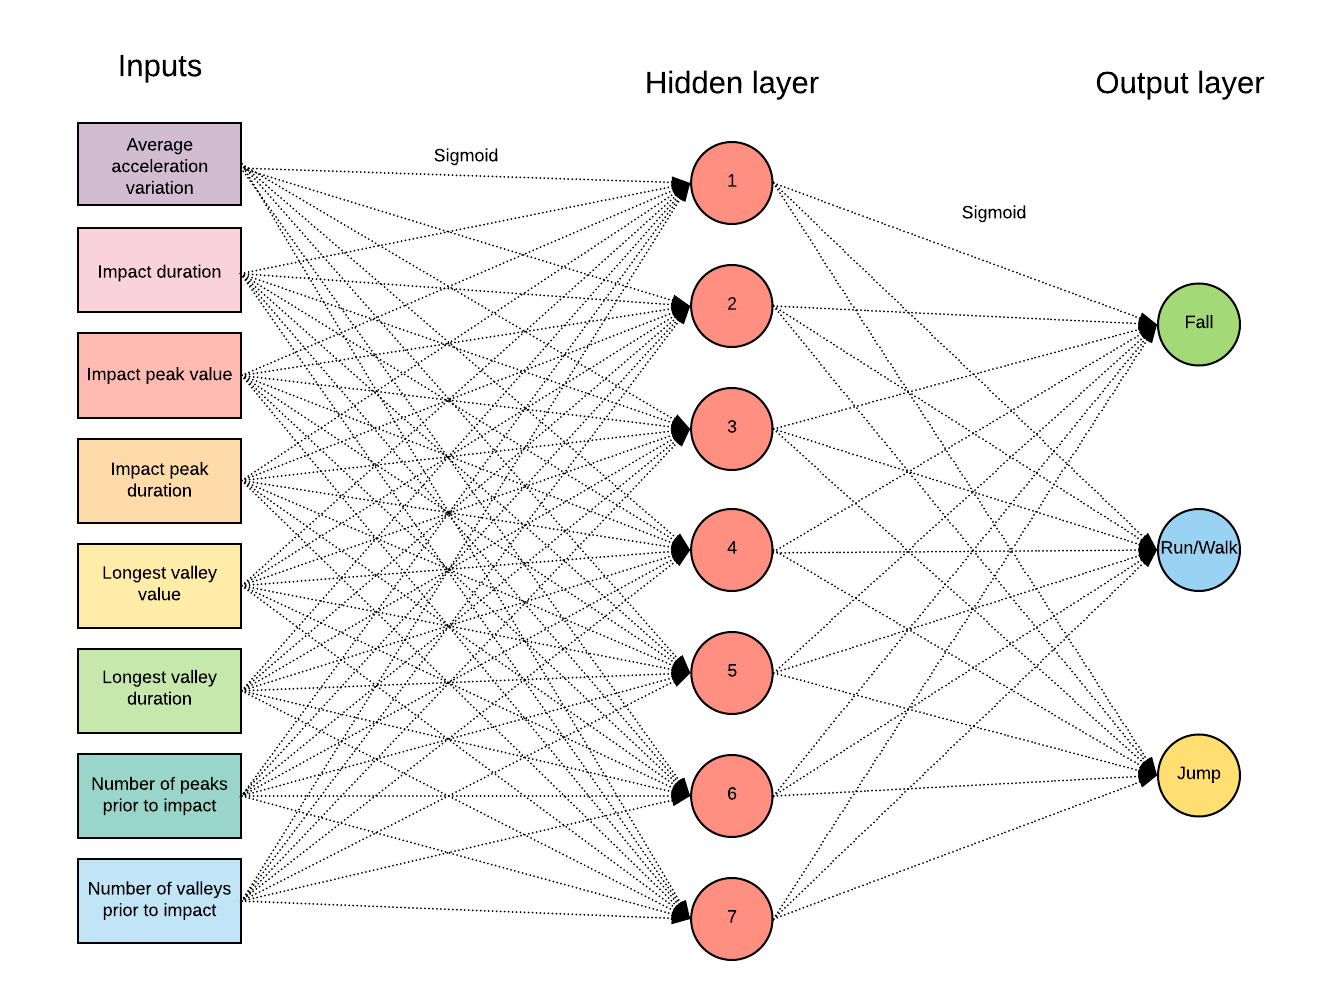
\includegraphics[width=15cm]{../img/neural-network-model.png} }}%
				\caption{The neural network}%
				\label{fig:neural-network}%
			\end{figure}

		\subsubsection{Training the model}
			When training the model, we downloaded all the data samples from the database and printed them to a CSV-file using our stand alone graphical utility tool. The dataset is then split up between training-set, and evaluation-set on a ratio of 9:1. The training set contains the labeled training data whereas the evaluation-set contains unlabeled data for measurement and cross-validation. The network training program uses the commonly used feed-forward <-> back-propagation method \cite{neural_networks} to fit the model. 

		
		\subsubsection{Using the model}
			The trained and evaluated neural network are finally converted into two separate file formats that can be used natively in iOS and Android applications. The generated files are simply included in the mobile application project after what they can be used to make predictions on future real life events. The input to the models are a vector of length eight, containing the values of the eight features for an event extracted by the feature-extractor. The output is a vector of length three, containing the independent probabilities of class adherence for the same event. 
			
			In the final product, where data collection functionality is removed, it is the values in the output vector that are used to finally decide if an event are to be classified as a fall accident or not. If the probability that the event belongs to the fall-class exceeds the other two, the application flags the event as a fall and presents the discard screen to the user, otherwise, the event will be automatically discarded by the application. 

\bibliography{bib_peter}
\bibliographystyle{ieeetr}

\end{document}